\chapter{Experimental Design}
This chapter document the concepts and technical approaches used in this thesis, as well as procedural concepts for understanding the experiments of this thesis.

\section{Experimental Design Overview}
	\paragraph{Thesis Goals} The central goal of this thesis's experiments is to compare size and speed of different author detection methods against the effectiveness of those same author detection methods on a resource constrained device such as a mobile phone.  Size and speed are critical to this thesis. This is due to the restrictive nature of mobile phones.  However, the nature of these experiments allows the results to be applied to other computing platforms with limited resources such as nano-computers, mobile sensors, or yet unimagined devices.
	\paragraph{Experimentation Phases}To achieve the thesis goal, experimentation will be conducted in two phases: parameter evaluation and mobile phone performance evaluation.  In parameter evaluation, the effectiveness of different combinations of classification methods, features sets, group sizes, and smoothing/filtering to compare prediction performance against model size and processing requirements.  During the mobile phone performance evaluation, the combinations of classification methods that are both feasible and effective are used on mobile phones to determine the overall performance and impact of running author detection on an actual mobile phone.

\section{Phase One: Parameter Evaluation} This phase will evaluate numerous combinations of two classification methods, five feature sets, six grouping sizes, three grouping methods, and two corpora to determine the computing requirements and effectiveness of these combinations.  Preparing for these evaluations takes several steps including determining the required combinations, organizing and compressing the feature references, preparing the training and prediction data, building the models, and, finally, running the prediction tests.  The results for all prediction test will be stored in a mySQL database which will also store the resulting f-score, precision, recall, and size of model for each test.

	\subsection{Creating the Testing Combinations} The classification methods to be compared are Naive Bayes and Support Vector machines (SVM). Naive Bayes is fast and uses a relatively small amount of RAM and disk storage. SVMs, are slower, use greater RAM and disk storage, but often yield higher f-scores.  There are numerous feature sets that can be chosen.  For this thesis, 1-grams, 2-grams, 5-grams, gappy bigrams, and orthogonal Sparse bigrams will be examined.  The intuition is that 1-grams are simple and use less space, but will be less effective than bigger feature sets such as gappy bigrams or 5-grams.
	\paragraph{} For this thesis, two feature reference sets will be examined, a bootstrapped bag of words and the Google Web1T corpus.  Bootstrapped bag of words simply means finding all the unique types within a training set and making each type a feature in the feature set. Since the Google Web1T corpus is huge, a parameter of that feature reference which can be adjusted is the percentage of a given feature set that might be used.  These experiments will permute through these numerous options to determine size, speed, precision and f-score.  The end result will be an analysis of the utility of these various approaches to author detection on a mobile phone.  A graphic of the parameter combinations is given in Figure \ref{fig:parameterCombinations}.   
	
	\begin{figure}[ht!]
		\begin{center}
			\fbox{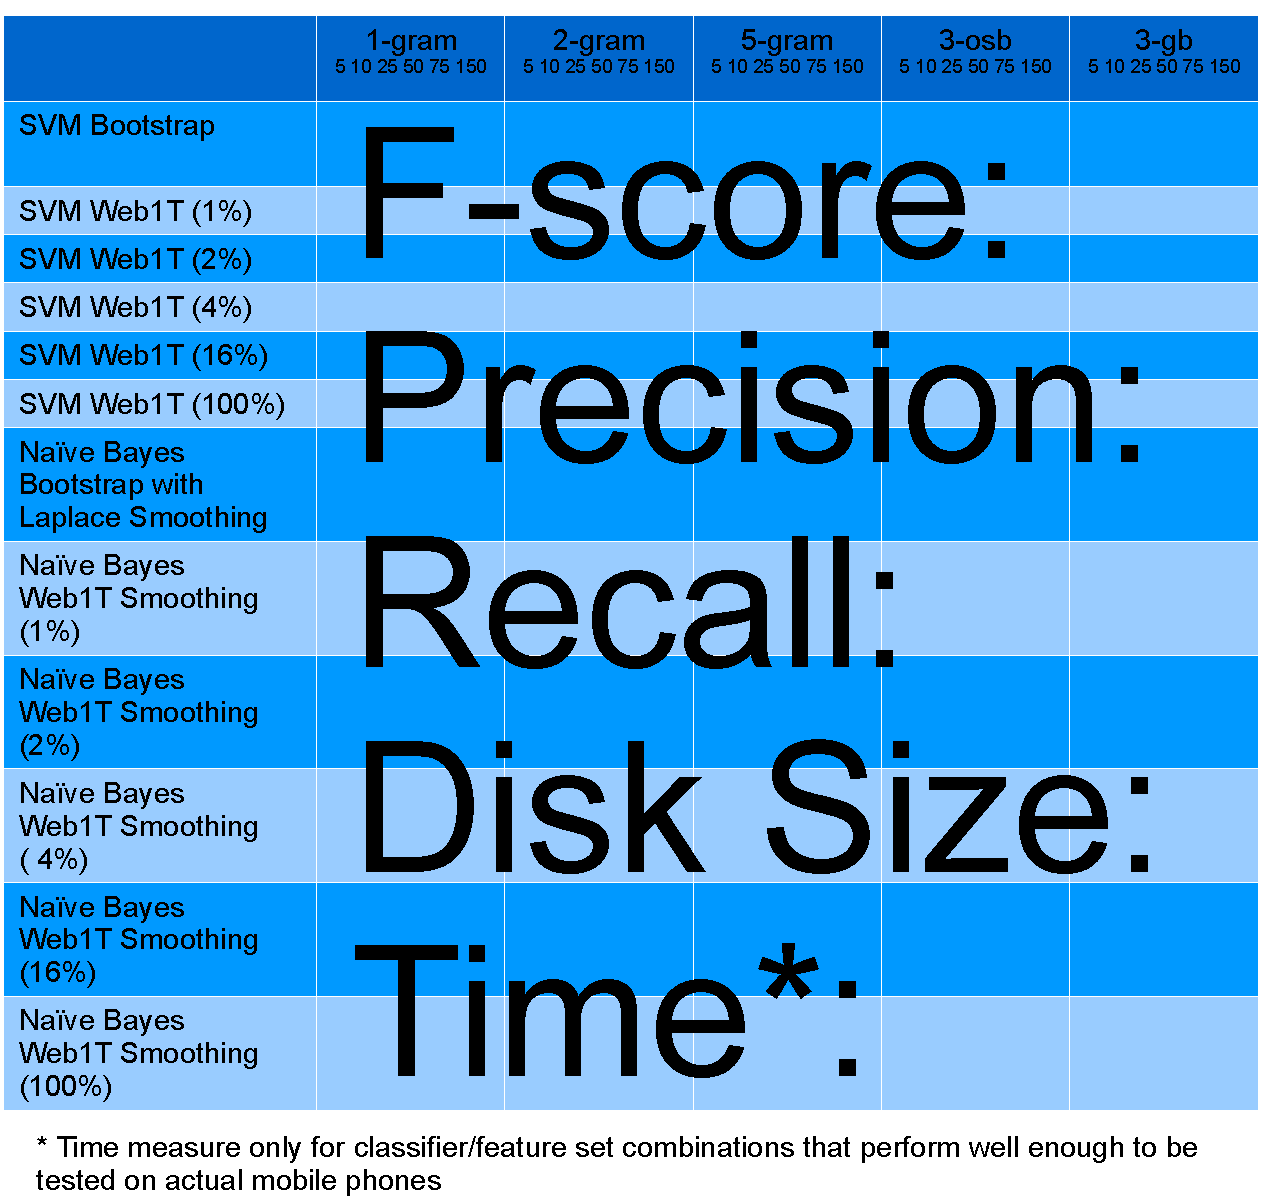
\includegraphics[width=0.5\textwidth]{Experiment_Design.pdf}}
			\caption{Parameter Combinations for Testing}
			\label{fig:parameterCombinations}
		\end{center}
	\end{figure}
	
The small numbers "5 10 25 50 75 150" given under each column heading in Figure \ref{fig:parameterCombinations} indicate that all authors will be tested in groups of 5, 10, 25, 50, 75, and 150 using three different grouping strategies: small-to-large, small-and-large, and random. In small-to-large, the authors with the smallest amount of training data are grouped together.  In small-and-large, small authors and large authors are paired together.  In the random grouping, the authors are grouped together by a pseudo-random selection.  The reasoning for these three grouping strategies is to provide insight into the effect of prolific authors versus less prolific authors.  If results are similar for the same author for each group, the prolific writing may not impact the outcome of author detection with these methods.  This is needed information to rule out that the test author detection methods simply select the most prolific author instead of the actual author.

	\subsection{Organizing and Compressing Feature References} A key element to this testing is the use of the Google Web1T corpus.  The Web1T corpus contains billions of types with a token mass of just over 1 trillion.  The size and breadth of the Web1T corpus makes it appealing as a source for smoothing in Naive Bayes and a tool for creating models in SVM. However, due to the huge size of the Web1T corpus, the text files comprising the corpus must be compressed and managed for use on desktop workstations, servers, and especially mobile devices.  Managing the corpus requires determining what portions of the Web1T corpus will be used.  Using the choice of 5-grams as an example for illustration purposes, suppose only the 5-grams portion of the Web1T corpus might be used.  The 5-grams constitutes 118 text files containing up to 10 million lines of text each. Each line of the Web1T 5-gram files contains space separated words (making up the type) followed by a count, separated from the words by a tab.  The lines of text are organized alphabetically by token where uppercase letters are distinct from lowercase letters. Even using only one size of gram from Web1T, a reverence of this size is slow and bulky for machine learning use.  Therefore, a subset of the reference is needed.
		\paragraph{Sizing the Feature Reference Set} To manage the size of Web1T, a small portion of the 5-grams could be chosen -- 1\%, 2\%, 4\%, etc.  To choose which part of the reference to use (largest, smallest, random) this thesis takes advantage of Zipf's Law.  Zipf's law states that the highest frequency word occurs approximately twice as often as the next most frequent word.  By that reasoning, a list of the types with the highest counts is needed to capture the largest use of words in a natural language corpus.  To get this count ordered list, the complete set of Web1T n-grams are recreated.  The recreated files list each type organized by count instead of alphabetically.  If two or more types have the same count, then those types are list alphabetically.  The types are still listed first as a group of space separated words followed by a tab and ended with a count.

		\paragraph{Three Tiered Hashing Scheme} Even once the feature set of types to be used for classification has been determined, the smaller set of text is still too slow to process and very bulky to store.  To further compress the data, a three tiered hashing scheme is used.  The structure of the three tiered hashing scheme is shown in Figure \ref{fig:3tierHashStructure}. 
		
		\begin{figure}[ht!]
			\begin{center}
				\fbox{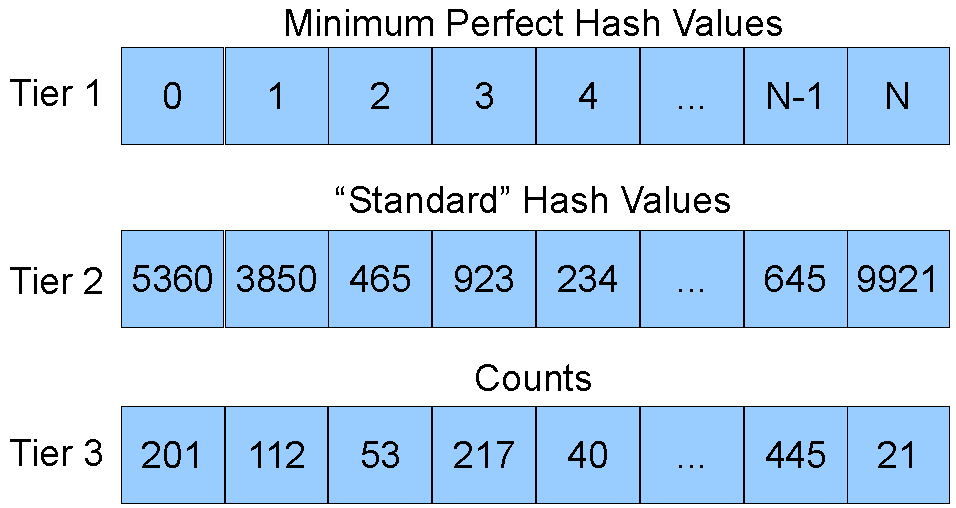
\includegraphics[width=0.75\textwidth]{3_tier_explanation.pdf}}
				\caption{Three Tiered Hashing Scheme Structure}
				\label{fig:3tierHashStructure}
			\end{center}
		\end{figure}
		
		The first tier is comprised of minimal perfect hash (MPH) values of the selected feature set.  The second tier of the scheme is comprised of a 64 bit hash of the original type.  This second tier's job is to reduce the probability of a false positive in the fist tier.  This issue arises because no matter what string is input to the MPH function, a valid MPH value will be produced.  The second tier's traditional hash is accessed by mapping the MPH value to the index of an array that comprises the second tier.  That array cell contains the 64 bit hash of the original text used to create the MPH value.  This make the false positive rate for a given type $\frac{1}{2^{64}} * \frac{1}{\text{range of MPH values}}$ which is deemed an appropriate risk of collision in this hashing scheme.  The third tier is simply an array of long values.  The MPH value from tier 1 is used to access this array which hold the count value for a given type.  An example of converting a phrase, "the quick brown", is shown in Figure \ref{fig:3tierHashExample}. 
		
		\begin{figure}[ht!]
			\begin{center}
				\fbox{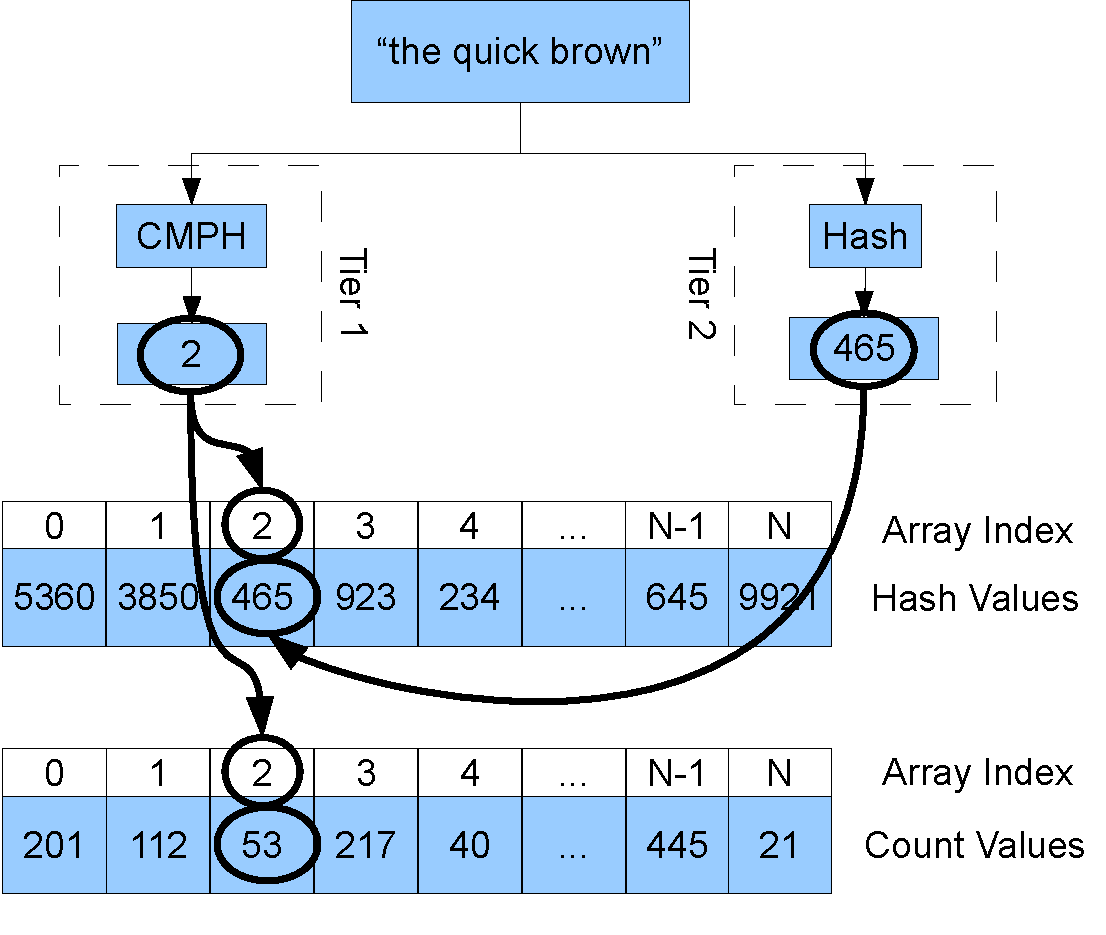
\includegraphics[width=0.75\textwidth]{3_tier_example.pdf}}
				\caption{Three Tiered Hashing Scheme Example}
				\label{fig:3tierHashExample}
			\end{center}
		\end{figure}
		
		These different tiers are not contained in a single data structures.  The MPH data structure, tier 1, is contained in a file called "keys.mph".  The array of hash values, tier 2, is contained in a file called "signature".  The counts are contained in a Java object file call LongCountsArrayFile.  The Naive Bayes experiments use all three tiers of this structure for smoothing values.  The SVM experiments only use tier 1 and tier 2 to verify that a string encountered actually belongs to the feature set.  These hefty data files comprise the bulk of storage required on the mobile device.  Since these data files get loaded into RAM during the prediction process, the file sizes also impact RAM requirements. The impact on RAM and disk storage makes management of the size of keys.mph, signature, and LongCountsArrayFile an important aspect of the experiments.

		\paragraph{Choosing Artifacts for the Three Tiered Hashing Scheme} One impact of using MPH to reduce the size of storing types is a loss of flexibility with the text artifact selection process.  Before the MPH data structure is created, the creator must determine if punctuation, capitalization, sentence boundaries, or "unknown" words will be allowed.  The omission of each of these artifact types brings its own unique challenges. A binary style number scheme was adopted for each of these features where capital letters hold the 1 position, punctuation the 2 position, unknown word tags the 4 position, and sentence boundaries hold the 8 position.  The complete matrix of artifacts allowed in the MPH model is included in Figure \ref{fig:cmphMatrix}.
		
		\begin{figure}[ht!]
			\begin{center}
				\fbox{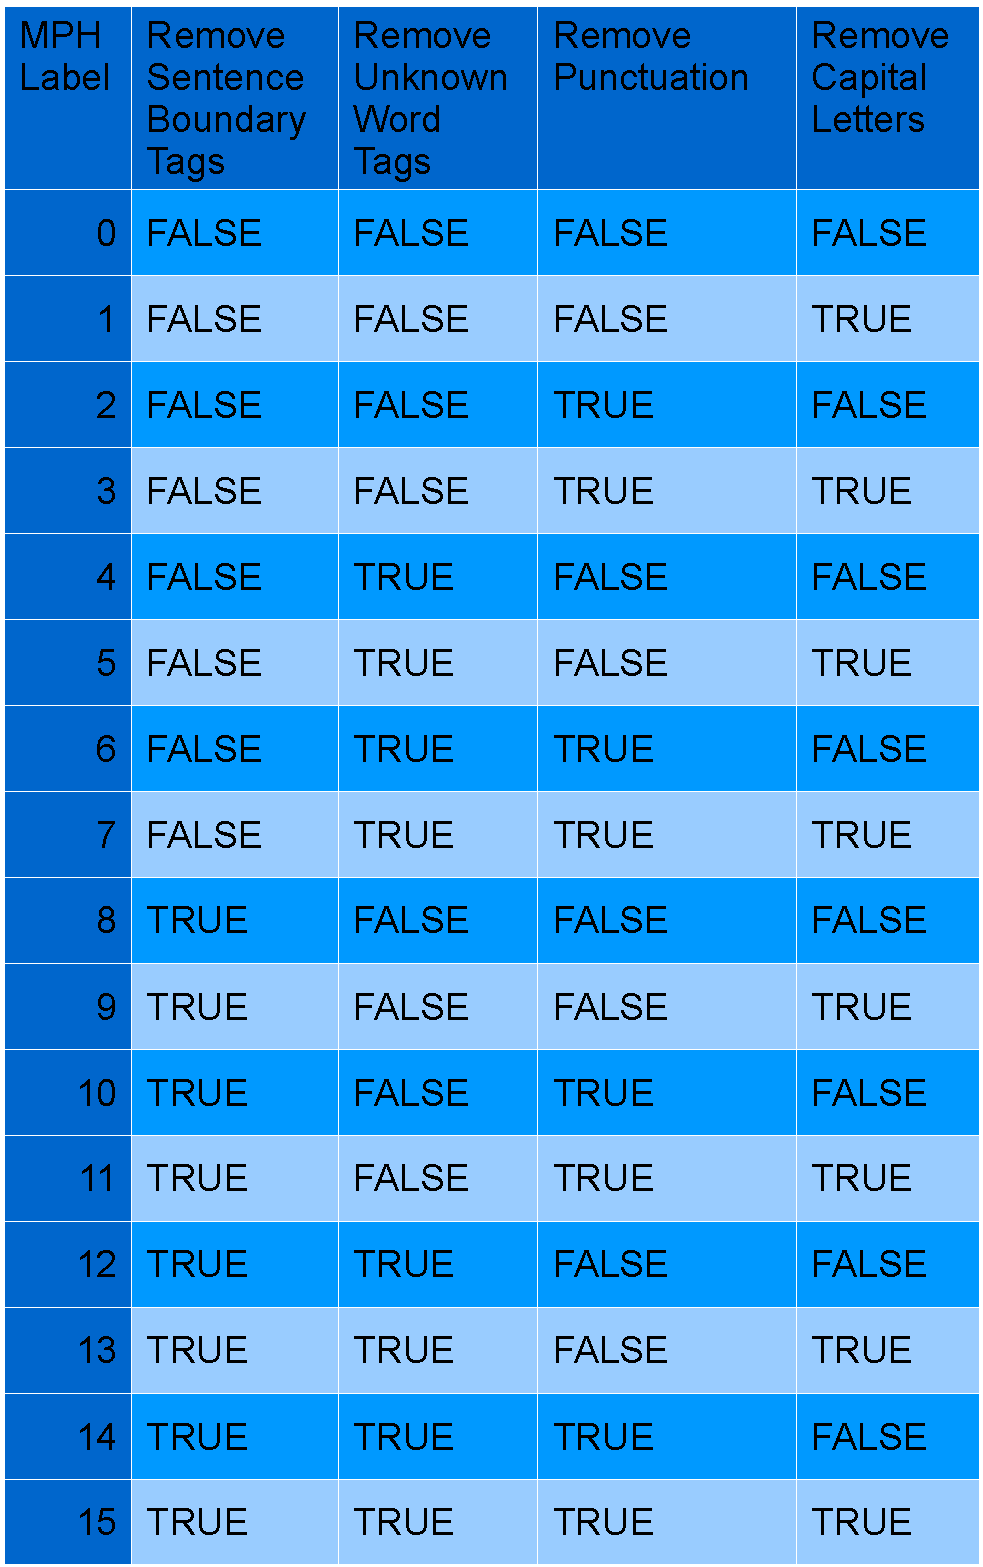
\includegraphics[width=0.5\textwidth]{cmph_matrix.pdf}}
				\caption{Matrix of CMPH Models by Artifacts Included}
				\label{fig:cmphMatrix}
			\end{center}
		\end{figure}
		
			\subparagraph{Omitting Punctuation} Omitting punctuation provides two options for dealing with the corpus: replace punctuation with "$<\text{UNK}>$" or drop the punctuation altogether.  If punctuation is dropped, then any type containing a punctuation mark in the feature reference set must be completely ignored.  If the punctuation is replaced with $<\text{UNK}>$, then a search within the existing count structure must be conducted for a corresponding entry for $<\text{UNK}>$ and any non-punctuation words in the type.  While dropping punctuation is much simpler to implement than employing "$<\text{UNK}>$" tags, however, Google did count punctuation as a word in type construction, so correlation between n-gram counts in the Web1T corpus and the trained/predicted documents is slightly affected. To maintain simplicity, the simple drop approach was used in these experiments.
			\subparagraph{Omitting Capitalization} Omitting capitalization is straightforward for construction of tier 1 and tier 2, the inputted text for the type is converted to all lower case and a check is conducted to see if that type is already in the MPH data structure.  For tier 3, which contains the counts, the lower case versions of the word must have its count mass added with its corresponding uppercase types.  This adds complexity to the insertion process for MPH but is easily managed.  Another option would be to simply drop all types that contained capitalization, but that would remove a large count mass from the Web1T corpus.  Adding counts was the method used in this thesis to deal with omitting capitalization.
			\subparagraph{Omitting Sentence Boundaries}  Sentence boundaries are denoted in the Web1T corpus as $<\text{S}>$ and $<\backslash \text{S}>$. Dropping sentence boundaries is straightforward since there is no replacement or count mass issues to deal with.  Since the tools for locating sentence boundaries make use of their own machine learning processes, no sentence boundaries were used in these experiments.
			\subparagraph{Omitting Unknown Words} In the Web1T corpus, "unknown" words have a specific meaning.  To be included in any corpus n-gram set, a word must have appeared as a 1-gram at least 200 times in the Google database.  By contrast, to be 2-gram, 3-gram, 4-gram, or 5-gram, that gram had to appear at least 40 times in the Google database.  This created as situation where a word would need to appear in a 2-or-higher-gram, but was not allowed into the corpus because it did not appear 200 times in the overall database.  Words that fall into that category are replaced with the tag $<\text{UNK}>$ in the Web1T corpus.  Removing $<\text{UNK}>$ words from the MPH has no effect on the counts in tier3 and is a straightforward process.
		
		\paragraph{Choosing N-Grams} N-grams can be as small as a 1-gram and grow, theoretically, to any size N imaginable.  The preferred reference set for this thesis, the Web1T corpus, uses 1, 2, 3, 4, and 5-grams.  While it is tempting to test all 5 N-gram sizes available in the corpus, only three were used.  1-grams and 5-grams were chosen to represent opposite ends of the size N gram spectrum available.  2-grams were used as a strong comparison to gappy bigrams and orthogonal sparse bigrams discussed below.  Future work could focus on 3 and 4-grams to determine if there is a performance to size advantage in using those size of N-grams.
		
		\paragraph{Gappy Bigram and Orthogonal Sparse Bigram Construction} Once the 3 tier structure is created and functional, there are still two type of features remaining to be created.  The Web1T corpus only contains standard n-grams, not gappy bigrams or orthogonal sparse bigrams.  To create these more exotic types of bigrams, a rule for counting distance and a notation scheme was needed.  It was decided to use "lesser included counts" for both the gappy bigrams and the orthogonal sparse bigrams.  This means that a word1 word2 pair would count for osb-0, osb-1, osb2, etc.  While previous papers placed the distance for an OSB between word1 and word2 \cite{bikel_if_2007}, this thesis constructed the OSBs with the distance after word2 for easier parsing.  The gappy bigrams and OSBs were constructed from the 2, 3, 4, and 5-grams in the Web1T Corpus.  Word pairs from a distance of 0 (a traditional bigram or an OSB-0) to a distance of 3 (an OSB-3 or the first and last word in a 5-gram) were built from the Web1T corpus.  This process only looks at the first and last words in a 3-gram, 4-gram, or 5-gram since the inner words of this gram are already captured in the 2-gram.  Using the inner 2-grams would double count 2-grams and throw off the count mass.  The same is true for 3-grams inside of 4 and 5-grams as well as 4-grams inside of 5-grams.
	
	\paragraph{Grouping By Size} With references built and sized, an efficient structuring of the authors and documents needs to be devised.  During data file construction, the grouping and conversion processes happened simultaneously.  The grouping sets built were: small-to-large, small-and-large, and random.  
		\subparagraph{Small-To-Large} The small-to-large group matched the least prolific authors together with increasing size up to the most prolific authors.  For example, of the 5 authors in the ENRON corpus with 5 total kilobytes worth of text are group together while the 5 authors with greater than 1 total megabyte of text are group together.  No author is picked more than once.  An example is shown in Figure \ref{fig:smallToLargeGrouping}.
		\begin{figure}[ht!]
			\begin{center}
				\fbox{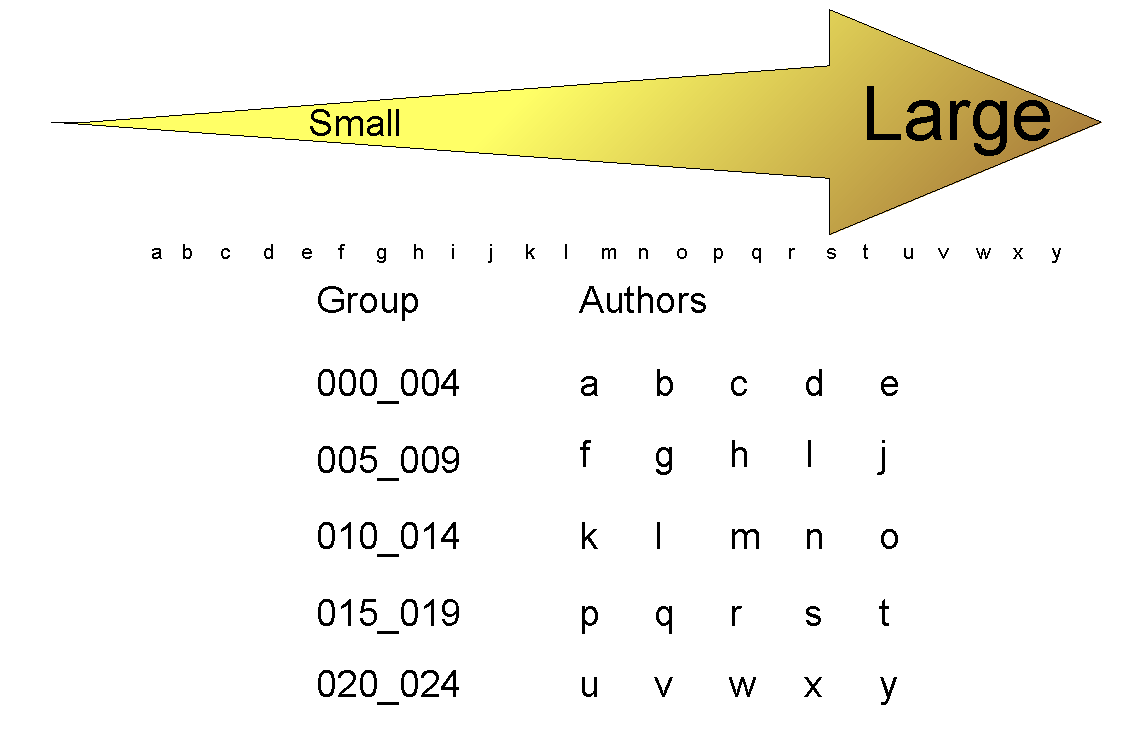
\includegraphics[width=0.5\textwidth]{small_to_large_grouping.pdf}}
				\caption{Small-To-Large Group for Group Size 5, 25 Authors}
				\label{fig:smallToLargeGrouping}
			\end{center}
		\end{figure}
		\subparagraph{Small-And-Large} The next group, small-and-large, is created by binning the authors by size.  Then one author from each bin is picked to be group with one author from each other bin.  For example the least prolific author is paired with one author from the most prolific bin and one author from each bin in between.  In this situation, the selection from each bin is not random.  The least prolific remaining author from each bin is picked for grouping.  No author is picked more than once. An example is shown in Figure \ref{fig:smallAndLargeGrouping}.
		\begin{figure}[ht!]
			\begin{center}
				\fbox{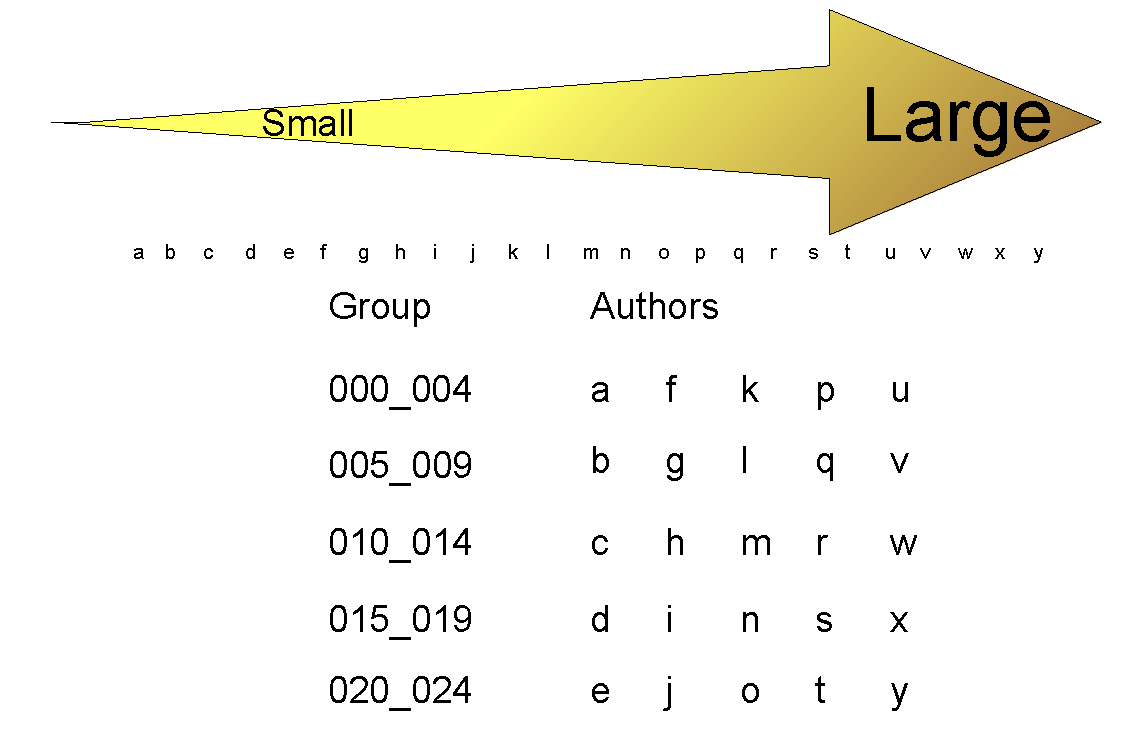
\includegraphics[width=0.5\textwidth]{small_and_large_grouping.pdf}}
				\caption{Small-And-Large Group for Group Size 5, 25 Authors}
				\label{fig:smallAndLargeGrouping}
			\end{center}
		\end{figure}
		\subparagraph{Random} This grouping simply produces a random number in the range of available authors and places the selected author into a group until that group is full.  Then the next group is filled the same way until no authors remain.  No author is picked more than once. No author is picked more than once. An example is shown in Figure \ref{fig:randomGrouping}.
		\begin{figure}[ht!]
			\begin{center}
				\fbox{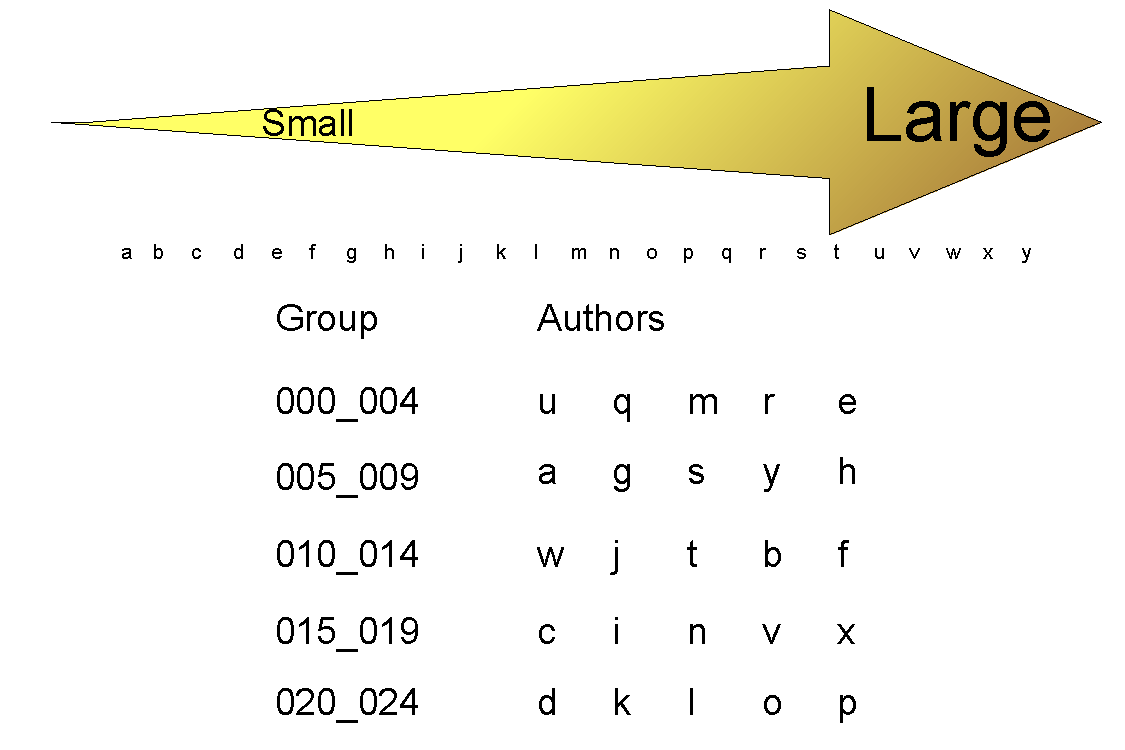
\includegraphics[width=0.5\textwidth]{random_grouping.pdf}}
				\caption{Random Group for Group Size 5, 25 Authors}
				\label{fig:randomGrouping}
			\end{center}
		\end{figure}
		\subparagraph{Group Sizes} Based on having 150 authors in the ENRON Corpus, the six following group sizes were used: 5, 10, 25, 50, 75 150.  These six group sizes coupled with the three grouping types, small-to-large, small-and-large, and random creates 18 grouping types.  Examples of these grouping types are 5 small-to-large, 5 small-and-large, 5 random, 10 small-to-large, ..., 150 small-to-large, 150 random.  Although using all 150 authors in a grouping set makes the procedure of how the 150 were grouped redundant, all three size 150 tests were conducted as a check on the experiments. If the 150 author grouping provides different reslts, then there may be an issue with the classifiers.
		\subparagraph{}After these grouping types were constructed, there were 171 totals sets (30 sets of 5 small-to-large, 15 sets of 10 small-to-large, ..., 1 set of 150 small-to-large, 1 set of 150 random.)  Each of these sets were intended to be run through Bootstrapped SVM, Web1T SVM, Laplace Smoothed Naive Bayes, and Web1T Smoothed Naive Bayes.  Assuming that only one MPH model is chosen to represent Google Web1T, that results in 684 experiments.  Since there are 16 different MPH models based on the combinations punctuation, capitalization, sentence boundaries, and unknown words, the number of experiments could rise drastically.  However, only two MPH models will be used during the experiments resulting in only 1,368 per feature type.  Using 1-grams, 2-grams, 5-grams, 3-gb, and 3-osb results in 6,840 totals experiments.
	
		\paragraph{Data File Format}With combinations of features, artifacts, and group sizes chosen and the MPH data structures created, the actual documents must be converted into a format that can be used by the classifiers. The LibSVM file format was used since that it is the native format for LibLinear, the tool used for SVM in this thesis.  The Naive Bayes classifier was built specifically for this thesis and was designed to use LibSVM format for convenience. The format of the data files consisted of an integer representing the author followed by a space, followed by a number representing the MPH value, followed by a colon, followed by another number representing the count.  Each succeeding instance of a MPH value coupled with a count is separated by a space.  Each document in the corpus is represented by a single line.  Each line's mph number is in increasing order from left to right.  The data files store the word/count pairs in a sparse fashion.  This means that a zero count is not included in the data file.  Absence of a word/count pair constitutes a zero count without needlessly using up space in the file.  An example of this file format is provide in Figure \ref{fig:svmFormat}.
		\begin{figure}[ht!]
			\begin{center}
				\fbox{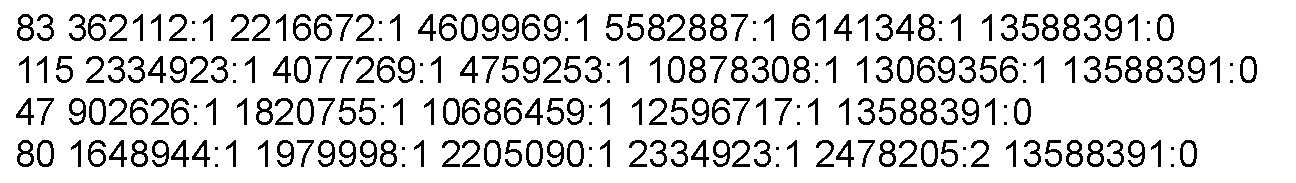
\includegraphics[width=.75\textwidth]{svm_format.pdf}}
				\caption{LibSVM File Format}
				\label{fig:svmFormat}
			\end{center}
		\end{figure}
	
	\paragraph{Running SVM} With the data files created, the classifiers can be applied. The chosen tool for author detection using SVM is LibLinear.  LibLinear was chosen for its speed compared to LibSVM.  The LibLinear source code was slightly modified to allow training a model from a data set, then running prediction on a separate set without using the built-in cross validation function.  During the training phase, each author has a SVM model built for it from a training file in a directory labeled "train".  During the prediction phase, document contained in another file are used to predict the mostly likely author.  That file is contained in a folder called "predict". The SVM author result is printed to a result file in a directory labeled "result".  The f-score, precision, and recall for each file is recorded in a file inside a folder labeled "analysis".  The analysis file also contains a full confusion matrix, time of prediction, size of original file, and other statistics.  This file is finally pulled into a mySQL database for storage and calculation of precision, recall, and f-score..
	\subparagraph{} The size of the author models impacts RAM usage and disk space.  LibLinear stores SVM models as an array. RAM and storage are not the only limits.  An array of integers representing token counts can be sizable, especially when token counts are long numbers (64 bits) instead of integers (32 bits). 
	\subparagraph{} RAM and disk storage are not the only limits. By specification, arrays in Java are limited to $2^{31}-1$ entries.  This means the model cannot contain more than $2^{31}-1$ features.  Also, the model must be loaded into RAM, so the number of authors coupled with the size of the author model must be weighed against the available RAM and disk storage.
	
	\paragraph{Running Naive Bayes} The Naive Bayes classifier has been specifically built for this thesis.  The classifier reads in a pre-built array of long values from a file.  The two types of arrays are a Laplace Smoothing array, which is comprised of all 1's.  the second type of array is the Google Smoothing array comprised of the count values from the Web1T corpus.  Using an array to hold the smoothing values for Naive Bayes has an impact on RAM usage.  There must be enough available RAM to hold the smoothing array.  To prevent having numerous copies of the smoothing array in memory (one for each author being trained) a hashmap is used to create the author models instead.  The process for training put each encountered feature type into a hashmap along with a count of $1 plus \text{the array smoothing value}$.  If that feature type is encountered, the the count is simply incremented. Once all the training documents have been read and counted, the hashmaps of feature types and counts is converted into a hashmap of feature types and log of probability.
	\paragraph{}During the prediction process, each encountered feature type is queried against the author hashmap first.  If the feature type is found in the hashmap, then the hashmap $\log{probability}$ is used.  If not, then the smoothing array containing log of probabilities is used.  An example of this hashmap/array process is shown in Figure \ref{fig:predictionFlowChart}. The result of the prediction process is outputted to a file in the corresponding results directory.  Those results are then processed into a file in the corresponding analysis folder where all data is then read into a mySQL database for evaluation of precision, recall, and f-score.
		\begin{figure}[ht!]
			\begin{center}
				\fbox{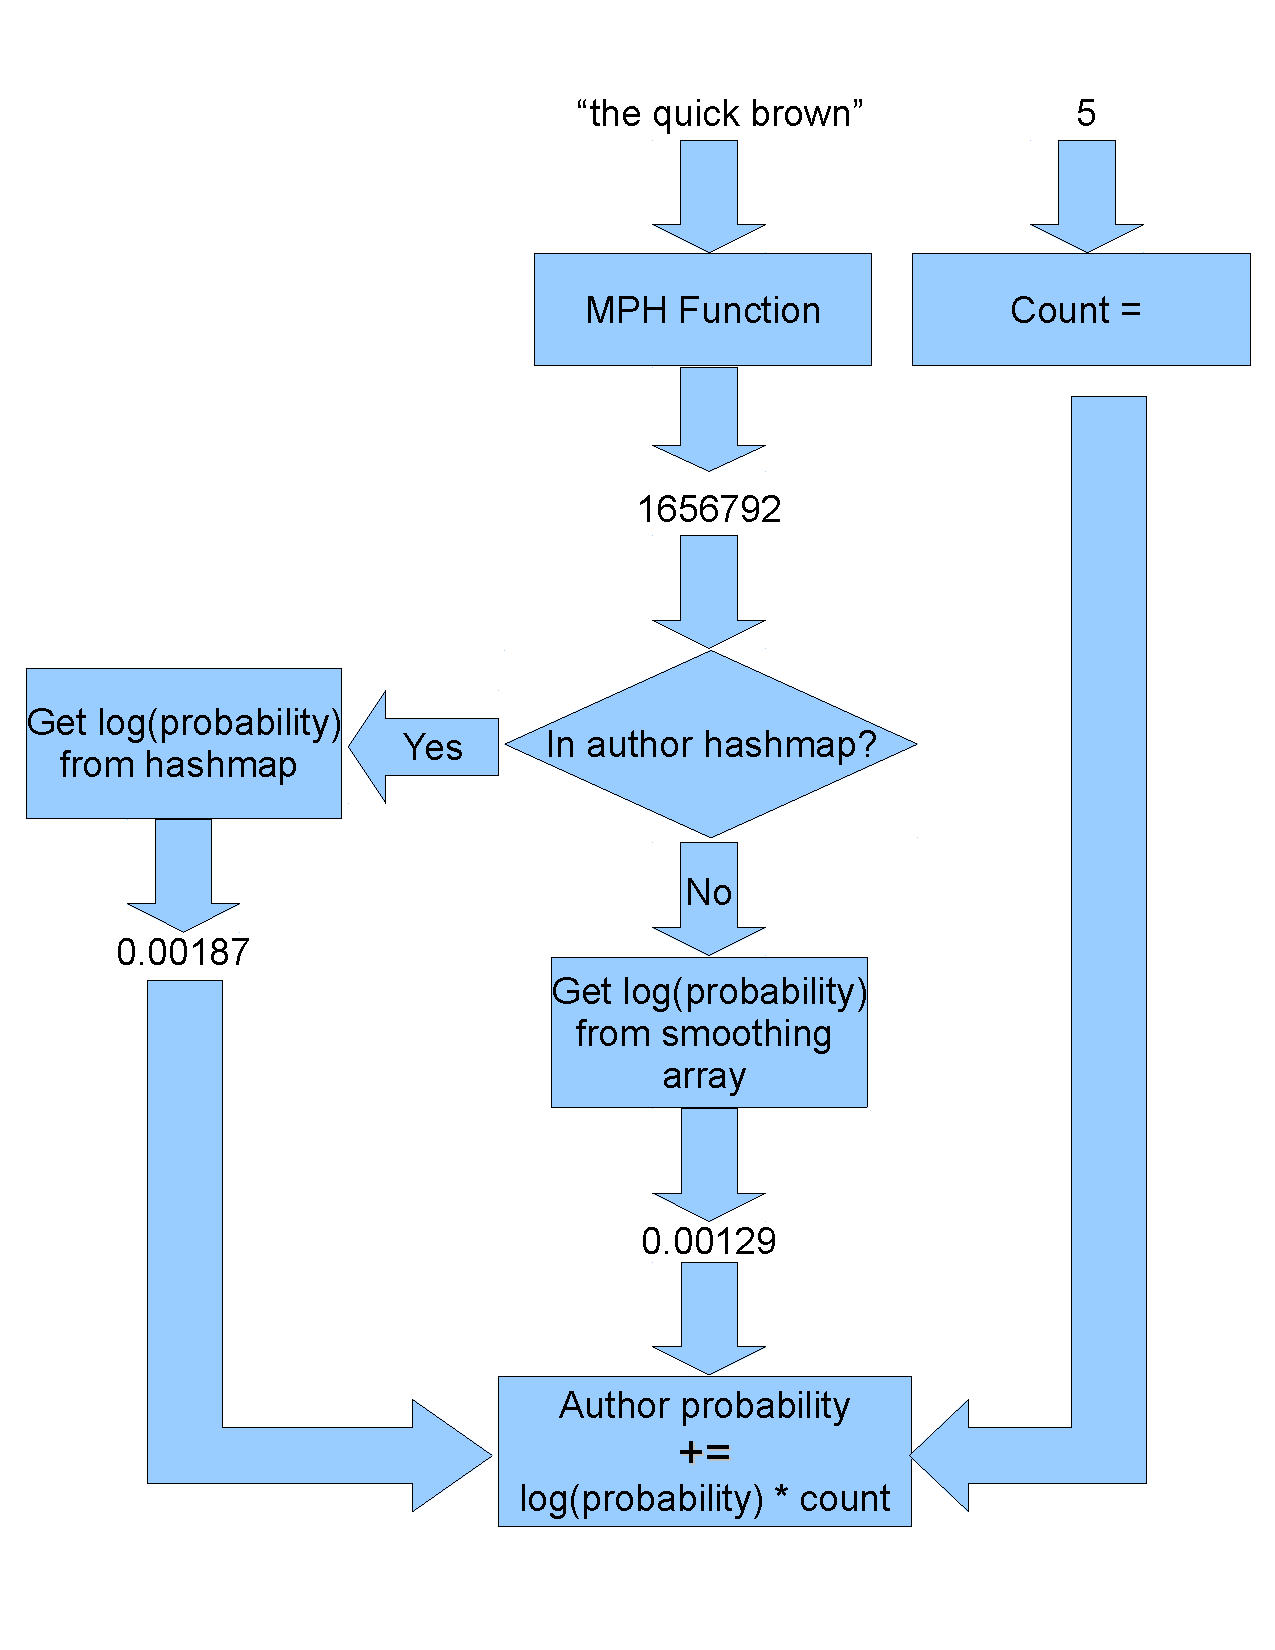
\includegraphics[width=.75\textwidth]{prediction_flow_chart.pdf}}
				\caption{Naive Bayes Hashmap and Smoothing Array Flow Chart}
				\label{fig:predictionFlowChart}
			\end{center}
		\end{figure}

%\section{Experiment Design}
%	\paragraph{}The objective of the experiments in this thesis are to populate a table of key metrics regarding author detection on a mobile phone.  The keys metrics are f-score, precision, recall, size on disk, %size in RAM, CPU consumption, and time required.  These metrics are aimed at the process of predicting the author, not at the process of training for the authors.  All author detection model training will be conducted on a workstation or server, not on a mobile phone.  The experiment will use a variety of combinations of feature sets, classification methods, and user set sizes.  The specific combinations are given in ;adslkfjads;lfkjads;lfk below:
%	\begin{center} 
%		Corpora
%		\begin{itemize}
%			\item ENRON Email Corpus
%			\item Naval Postgraduate School Twitter Corpus
%		Classification Methods
%		\begin{itemize}
%			\item Naive Bayes with Laplace Smoothing
%			\item Naive Bayes with Google Web1T Count Smoothing
%			\item Support Vector Model bootstrapped from training set
%			\item Support Vector Model with Google Web1T Types for dimensions
%		\end{itemize}
%		Feature Sets
%		\begin{itemize}
%			\item 1-grams (unigrams)
%			\item 2-grams (bigrams)
%			\item 5-grams
%			\item 3-gappy bigrams
%			\item 3-orthogonal sparse bigrams
%		\end{itemize}
%		User Set Size
%		\begin{itemize}
%			\item all versus all (mutlicalss
%			\begin{itemize}
%				\item 5 users
%				\item 10 users
%				\item 25 users
%				\item 50 users
%				\item 75 users
%				\item 150 users
%			\end{itemize}
%			\item one versus all
%			\begin{itemize}
%				\item 5 users
%				\item 10 users
%				\item 25 users
%				\item 50 users
%				\item 75 users
%				\item 150 users
%			\end{itemize}

%\paragraph{}The two classifiers chosen were Naive Bayes and Support Vector Model.  While there are many classifier tools available, these two methods were chosen for nominally being on the opposite end of the simplicity and effectiveness scales.  For text classification tasks, Naive Bayes is often less effective than SVM.  Naives Bayes is simpler to implement than SVM, so the tradeoff is simplicity versus effectiveness.  Naive Bayes is much lighter on CPU usage and time than SVM.  Both Naive Bayes and SVM can process training and predicting files in a sparse format, which saves on disk storage.  Naive Bayes must deal with zero probabilities stemming from a lack of training data to make the Bayes equation work out to something other than zero, and, more importantly, smoothing lessens the impact of the spiky nature of discrete data.  This smoothing is intended to provide a more reliable result.  For SVM, the SVM model can be created by only accepting words found in the actual training data or the features can be created from a feature reference, such as Google Web1T.  In the case of using a feature reference, SVM simply puts a value of 0 for each feature not provided a number in the training or prediction data.
%\section{Program Design}
%	\paragraph{}Write a cmph module to transform strings of words into numeric values.  Store those values in a file.  Have this module account for sentence boundaries, punctuation, capitalization, and unknown words.
%	\paragraph{}Transform corpus documents from a set of strings to a set of cmph created values, a different document corresponding to each cmph model (punctuation, .  Store the corpora in cmph numeric form.

%\section{Data Management}

\section{Phase Two: Android Implementation}
	\paragraph{}To manage files on the mobile device, a rudimentary file manager was built with a text viewer added.  A button was also added to the File Manager to execute prediction against a document on the phone.  An Android Service was also constructed that listens for incoming SMS messages.  When an SMS Message is "heard", it is processed for author detection.  The Service can be turned on and off using a button on the File Manager.  
	\paragraph{}To measure CPU and RAM impact caused by the author detection processing, the third party applications, and Memory Usage, was installed on the phones.  The method is to take a baseline of the phone's CPU and RAM usage with no Widgets or Applications running, the phone is attached to a recharging device, and no calls or texts are being sent.  The same phone conditions are being set for the processing tests where the only application that will run on the phone will be the SMS capture and author detection application for this thesis.  This will yield some basic metrics of author detection impact on the phone's capabilities.

\section{Corpora} Two corpora are used for this thesis: the ENRON Email Corpus and the Naval Postgraduate School (NPS) Twitter Corpus.  The aim of this thesis is to examine author detection using a mobile device.  Two of the most common text communications on a mobile device are email and SMS (texting).  The ENRON Email Corpus has been widely examined and has been used to author attribution in other studies.  This makes the ENRON Corpus a suitable standard to measure the author detection techniques used in this thesis.  The NPS Twitter Corpus is smaller and newer than the ENRON email corpus, but texting is extremely popular as a communications medium.  Determining the effectiveness of author detection over this rapidly expanding text standard is important for analyzing the effectiveness of author detection on mobile devices.
	\paragraph{ENRON Email Corpus} Each ENRON email was stored in a single text file within a folder labeled with the author's first initial, second initial, and last name.  Prior to processing each ENRON email, a systematic attempt was made to distill each email down into just the author's words.  To support this distillation, the email header was stripped from each email.  A search was conducted throughout the remaining text to find additional email headers.  These are the embedded headers caused by email replies and forwards.  Also to prevent biasing the author attribution, an attempt was made to systematically detect an email closing such as "Sincerely, Dave" or "Yours Truly, Jane".
	\paragraph{Naval Postgraduate School Twitter Short Message Corpus} All tweets from a single author were stored in a single text file.  Each tweet from that author was contained on its own line.  Each line begins with a date-time stamp with the content of the text following.  Prior to constructing the corpus, all "re-tweets" were removed to ensure the text came from a single author, not just from a single Twitter account.
	
\section{Intended Comparison}  Once all tests are complete, performance of the different combinations of feature and classifiers will be compared for both the ENRON email corpus and the Twitter Corpus.  This is to allow any differences in performance against the two primary media used on mobile phones.  The completed test results should provide insight into the possibility of author detection on a mobile phone against both email and short messages.




